\lab{SQL I: Introduction}{Introduction to SQL}
\objective{Being able to store and manipulate large data sets quickly is a fundamental part of data science.
The SQL language is the classic database management system for working with tabular data.
In this lab we introduce the basics of SQL, including creating, reading, updating, and deleting SQL tables, all via Python's standard SQL interaction modules.}

% TODO: reference https://docs.python.org/3/library/sqlite3.html.

% A database is a structured repository of data, and it allows for efficient storage and retrieval of information.
% A database is managed by a database management system, or DBMS.
% The most common DBMSs use a variant of the SQL language to interact with the database.

\section*{Relational Databases} % =============================================

A \emph{relational database} is a collection of tables called \emph{relations}.
A single row in a table, called a \emph{tuple}, corresponds to an individual instance of data.
The columns, called \emph{attributes} or \emph{features}, are data values of a particular category.
The collection of column headings is called the \emph{schema} of the table, which describes the kind of information stored in each entry of the tuples.
% See Figure \ref{fig:sql-relation} for an illustration of these ideas.

For example, suppose a database contains demographic information for $M$ individuals.
If a table had the schema \li{(Name, Gender, Age)}, then each row of the table would be a $3$-tuple corresponding to a single individual, such as \li{(Jane Doe, F, 20)} or \li{(Samuel Clemens, M, 74.4)}.
The table would therefore be $M\times 3$ in shape.
Another table with the schema \li{(Name, Income)} would be $M \times 2$ if it included all $M$ individuals.

% TODO: move this to SQL 2 where we talk about joins.
\begin{comment} % Primary keys (This got removed but is very important!)
Each table in a relational database must have at least one attribute that \textbf{uniquely} identifies an entry of the data, called a \emph{primary key}.
Most primary keys are ID numbers, but any attribute will do as long as the values are unique for each tuple.
For example, the \li{Name} attribute in the previous example could be considered a primary key provided no two individuals in the database have identical names.
\end{comment}

\begin{figure}[H]
    \centering
    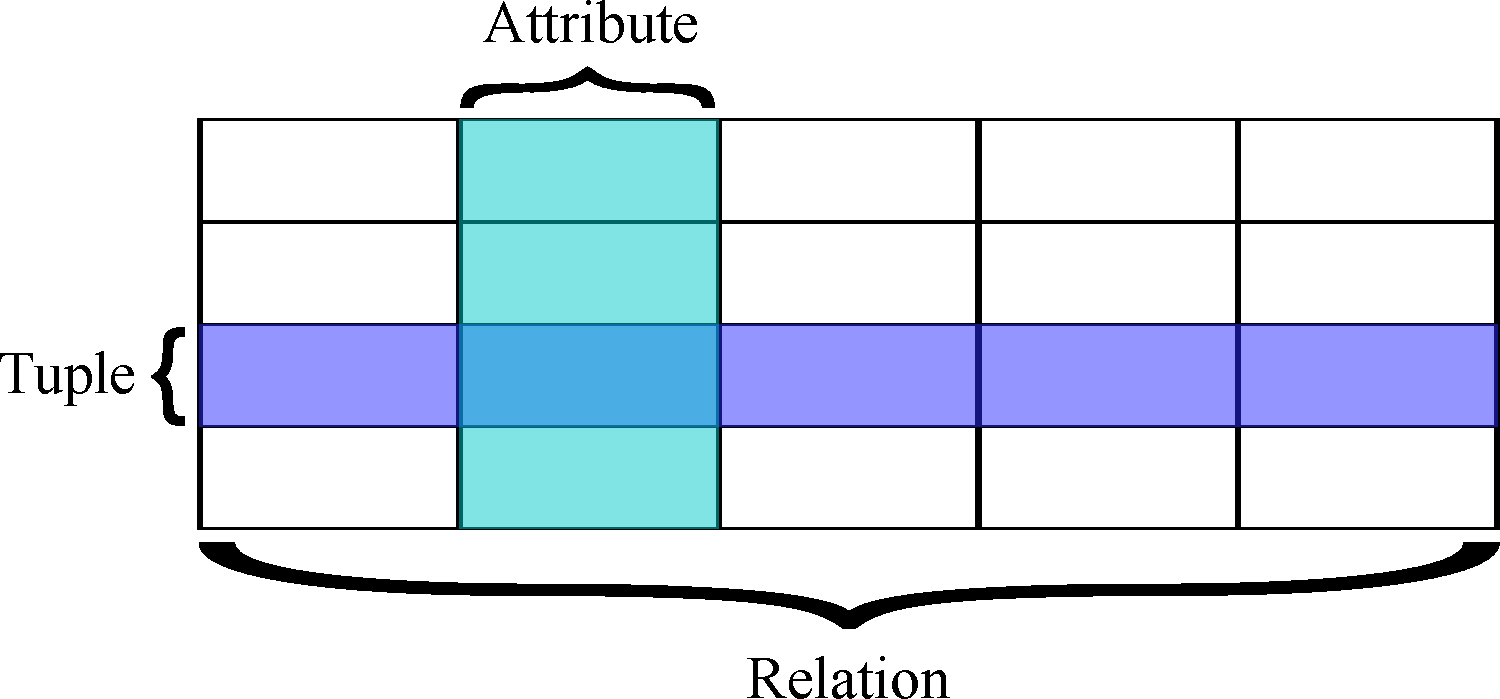
\includegraphics[width=.7\textwidth]{rdb_table.pdf}
    \caption{See \url{https://en.wikipedia.org/wiki/Relational_database}.}
    \label{fig:sql-relation}
\end{figure}

\subsection*{SQLite} % --------------------------------------------------------

The most common database management systems (DBMS) for relational databases are based on \emph{Structured Query Language}, commonly called \emph{SQL} (pronounced\footnote{See \url{https://english.stackexchange.com/questions/7231/how-is-sql-pronounced} for a brief history of the somewhat controversial pronunciation of SQL.} ``sequel'').
Though SQL is a language in and of itself, most programming languages have tools for executing SQL routines.
In Python, the most common variant of SQL is \emph{SQLite}, implemented as the \li{sqlite3} module in the standard library.

A SQL database is stored in an external file, usually marked with the file extension \texttt{db} or \texttt{mdf}.
These files should \textbf{not} be opened in Python with \li{open()} like text files; instead, any interactions with the database---creating, reading, updating, or deleting data---should occur as follows.

\begin{enumerate}
    \item Create a connection to the database with \li{sqlite3.connect()}.
    This creates a database file if one does not already exist.
    \item Get a \emph{cursor}, an object that manages the actual traversal of the database, with the connection's \li{cursor()} method.
    \item Alter or read data with the cursor's \li{execute()} method, which accepts an actual SQL command as a string.
    \item Save any changes with the cursor's \li{commit()} method, or revert changes with \li{rollback()}.
    \item Close the connection.
\end{enumerate}

\begin{lstlisting}
>>> import sqlite3 as sql

# Establish a connection to a database file or create one if it doesn't exist.
>>> conn = sql.connect("my_database.db")
>>> try:
...     cur = conn.cursor()                         # Get a cursor object.
...     cur.execute("SELECT * FROM MyTable")        # Execute a SQL command.
... except sql.Error:                               # If there is an error,
...     conn.rollback()                             #  revert the changes
...     raise                                       #  and raise the error.
... else:                                           # If there are no errors,
...     conn.commit()                               #  save the changes.
... finally:
...     conn.close()                                # Close the connection.
\end{lstlisting}

\begin{warn} % Remember to commit changes.
Some changes, such as creating and deleting tables, are automatically committed to the database as part of the cursor's \li{execute()} method.
Be \textbf{extremely cautious} when deleting tables, as the action is immediate and permanent.
Most changes, however, do not take effect in the database file until the connection's \li{commit()} method is called.
Be careful not to close the connection before committing desired changes, or those changes will not be recorded.
\end{warn}

The \li{with} statement can be used with \li{open()} so that file streams are automatically closed, even in the event of an error.
Likewise, combining the \li{with} statement with \li{sql.connect()} automatically rolls back changes if there is an error and commits them otherwise.
However, the actual database connection is \textbf{not} closed automatically.
With this strategy, the previous code block can be reduced to the following.

\begin{lstlisting}
>>> try:
...     with sql.connect("my_database.db") as conn:
...         cur = conn.cursor()                     # Get the cursor.
...         cur.execute("SELECT * FROM MyTable")    # Execute a SQL command.
... finally:                                        # Commit or revert, then
...     conn.close()                                #  close the connection.
\end{lstlisting}

\section*{Managing Database Tables} % =========================================

SQLite uses five native data types (relatively few compared to other SQL systems) that correspond neatly to native Python data types.

\begin{table}[H]
\begin{tabular}{c|c}
    Python Type & SQLite Type \\
    \hline
    \li{None} & \lsql{NULL} \\
    \li{int} & \lsql{INTEGER} \\
    \li{float} & \lsql{REAL} \\
    \li{str} & \lsql{TEXT} \\
    \li{bytes} & \lsql{BLOB}
\end{tabular}
\end{table}

The \lsql{CREATE TABLE} command, together with a table name and a schema, adds a new table to a database.
The schema is a comma-separated list where each entry specifies the column name, the column data type,\footnote{Though SQLite does not force the data in a single column to be of the same type, most other SQL systems enforce uniform column types, so it is good practice to specify data types in the schema.} and other optional parameters.
For example, the following code adds a table called \li{MyTable} with the schema \li{(Name, ID, Age)} with appropriate data types.

\begin{lstlisting}
>>> with sql.connect("my_database.db") as conn:
...     cur = conn.cursor()
...     cur.execute("CREATE TABLE MyTable (Name TEXT, ID INTEGER, Age REAL)")
...
>>> conn.close()
\end{lstlisting}

The \lsql{DROP TABLE} command deletes a table.
However, using \lsql{CREATE TABLE} to try to create a table that already exists or using \lsql{DROP TABLE} to remove a nonexistent table raises an error.
Use \lsql{DROP TABLE IF EXISTS} to remove a table without raising an error if the table doesn't exist.
See Table \ref{table:sql-table-management} for more table management commands.

\begin{table}[H]
    \begin{tabular}{c|l}
    Operation & SQLite Command \\ \hline
    Create a new table & \lsql{CREATE TABLE} \li{<table> (<schema>);} \\
    Delete a table & \lsql{DROP TABLE} \li{<table>;} \\
    Delete a table if it exists & \lsql{DROP TABLE IF EXISTS} \li{<table>;} \\
    Add a new column to a table & \lsql{ALTER TABLE} \li{<table>} \lsql{ADD} \li{<column> <dtype>} \\
    Remove an existing column & \lsql{ALTER TABLE} \li{<table>} \lsql{DROP COLUMN} \li{<column>;} \\
    Rename an existing column & \lsql{ALTER TABLE} \li{<table>} \lsql{ALTER COLUMN} \li{<column> <dtype>;} \\
    \end{tabular}
\caption{SQLite commands for managing tables and columns.}
\label{table:sql-table-management}
\end{table}

% TODO: include this in the discussion of Primary Keys in SQL 2.
% The \lsql{NOT NULL} command is a constraint on the StudentID column.
% It requires that all records in the table have a student ID.

\begin{info} % All caps and semicolons.
SQL commands like \lsql{CREATE TABLE} are often written in all caps to distinguish them from other parts of the query, like the table name.
This is only a matter of style: SQLite, along with most other versions of SQL, is case insensitive.
In Python's SQLite interface, the trailing semicolon is also unnecessary.
However, most other database systems require it, so it's good practice to include the semicolon in Python.
\end{info}

\begin{problem} % Create a student database.
Write a function that accepts the name of a database file.
Connect to the database (and create it if it doesn't exist).
Drop the tables \li{MajorInfo}, \li{CourseInfo}, \li{StudentInfo}, and \li{StudentGrades} from the database \textbf{if} they exist.
Next, add the following tables to the database with the specified column names and types.
\begin{itemize}
\item \li{MajorInfo}: \li{MajorID} (integers) and \li{MajorName} (strings).
\item \li{CourseInfo}: \li{CourseID} (integers) and \li{CourseName} (strings).
\item \li{StudentInfo}: \li{StudentID} (integers), \li{StudentName} (strings), and \li{MajorID} (integers).
\item \li{StudentGrades}: \li{StudentID} (integers), \li{CourseID} (integers), and \li{Grade} (strings).
\end{itemize}
Remember to commit and close the database.
You should be able to execute your function more than once with the same input without raising an error.

To check the database, use the following commands to get the column names of a specified table.
Assume here that the database file is called \texttt{students.db}.

\begin{lstlisting}
>>> with sql.connect("students.db") as conn:
...     cur = conn.cursor()
...     cur.execute("SELECT * FROM StudentInfo;")
...     print([d[0] for d in cur.description])
...
<<['StudentID', 'StudentName', 'MajorID']>>
\end{lstlisting}
\label{prob:sql1-create-student-tables}
\end{problem}

\section*{Inserting, Removing, and Altering Data} % ===========================

Tuples are added to SQLite database tables with the \lsql{INSERT INTO} command.

\begin{lstlisting}
# Add the tuple (Samuel Clemens, 1910421, 74.4) to MyTable in my_database.db.
>>> with sql.connect("my_database.db") as conn:
...     cur = conn.cursor()
...     cur.execute("INSERT INTO MyTable "
...                 "VALUES('Samuel Clemens', 1910421, 74.4);")
\end{lstlisting}

With this syntax, SQLite assumes that values match sequentially with the schema of the table.
The schema of the table can also be written explicitly for clarity.

\begin{lstlisting}
>>> with sql.connect("my_database.db") as conn:
...     cur = conn.cursor()
...     cur.execute("INSERT INTO MyTable(Name, ID, Age) "
...                 "VALUES('Samuel Clemens', 1910421, 74.4);")
\end{lstlisting}

\begin{warn} % SQL injection attack.
\textbf{Never} use Python's string operations to construct a SQL query from variables.
Doing so makes the program susceptible to a \emph{SQL injection attack}.\footnote{See \url{https://xkcd.com/327/} for an example.}
Instead, use parameter substitution to construct dynamic commands: use a \li{?} character within the command, then provide the sequence of values as a second argument to \li{execute()}.

\begin{lstlisting}
>>> with sql.connect("my_database.db") as conn:
...     cur = conn.cursor()
...     values = ('Samuel Clemens', 1910421, 74.4)
...     # Don't piece the command together with string operations!
...     # cur.execute("INSERT INTO MyTable VALUES " + str(values)) # BAD!
...     # Instead, use parameter substitution.
...     cur.execute("INSERT INTO MyTable VALUES(?,?,?);", values)  # Good.
\end{lstlisting}
\end{warn}

To insert several rows at a time to the same table, use the cursor object's \li{executemany()} method and parameter substitution with a list of tuples.
This is typically much faster than using \li{execute()} repeatedly.

\begin{lstlisting}
# Insert (Samuel Clemens, 1910421, 74.4) and (Jane Doe, 123, 20) to MyTable.
>>> with sql.connect("my_database.db") as conn:
...     cur = conn.cursor()
...     rows = [('John Smith', 456, 40.5), ('Jane Doe', 123, 20)]
...     cur.executemany("INSERT INTO MyTable VALUES(?,?,?);", rows)
\end{lstlisting}

\begin{problem} % Populate student tables.
Expand your function from Problem \ref{prob:sql1-create-student-tables} so that it populates the tables with the data given in Tables \ref{table:sql1-student-majorinfo}--\ref{table:sql1-student-grades}.

\begin{table}[H]
\begin{subtable}{0.55\textwidth}
    \centering
    \begin{subtable}{.45\textwidth}
        \centering
        \footnotesize
        \begin{tabular}{|l|l|}
            \hline MajorID & MajorName \\ \hline
            1 & Math \\
            2 & Science \\
            3 & Writing \\
            4 & Art \\ \hline
        \end{tabular}
        \caption{MajorInfo}
        \label{table:sql1-student-majorinfo}
    \end{subtable}
    \hfil
    \begin{subtable}{.45\textwidth}
        \centering
        \footnotesize
        \begin{tabular}{|l|l|}
            \hline CourseID & CourseName \\ \hline
            1 & Calculus \\
            2 & English \\
            3 & Pottery \\
            4 & History \\ \hline
        \end{tabular}
        \caption{CourseInfo}
        \label{table:sql1-student-courseinfo}
    \end{subtable}
    \\[1.em] % NOTE: Use 4.01em to align the tables at the top and bottom.
    \begin{subtable}{\textwidth}
        \centering
        \footnotesize
        \begin{tabular}{|l|l|l|}
            \hline StudentID & StudentName & MajorID \\ \hline
            401767594 & Michelle Fernandez & 1 \\
            678665086 & Gilbert Chapman & NULL \\
            553725811 & Roberta Cook & 2 \\
            886308195 & Rene Cross & 3 \\
            103066521 & Cameron Kim & 4 \\
            821568627 & Mercedes Hall & NULL \\
            206208438 & Kristopher Tran & 2 \\
            341324754 & Cassandra Holland & 1 \\
            262019426 & Alfonso Phelps & NULL \\
            622665098 & Sammy Burke & 2 \\ \hline
        \end{tabular}
        \caption{StudentInfo}
        \label{table:sql1-student-info}
    \end{subtable}
\end{subtable}
\hfil
\begin{subtable}{.35\textwidth}
    \centering
    \footnotesize
    \begin{tabular}{|l|l|l|}
        \hline StudentID & CourseID & Grade \\ \hline
        401767594 & 4 & C \\
        401767594 & 3 & B-- \\
        678665086 & 4 & A+ \\
        678665086 & 3 & A+ \\
        553725811 & 2 & C \\
        678665086 & 1 & B \\
        886308195 & 1 & A \\
        103066521 & 2 & C \\
        103066521 & 3 & C-- \\
        821568627 & 4 & D \\
        821568627 & 2 & A+ \\
        821568627 & 1 & B \\
        206208438 & 2 & A \\
        206208438 & 1 & C+ \\
        341324754 & 2 & D-- \\
        341324754 & 1 & A-- \\
        103066521 & 4 & A \\
        262019426 & 2 & B \\
        262019426 & 3 & C \\
        622665098 & 1 & A \\
        622665098 & 2 & A-- \\ \hline
    \end{tabular}
    \caption{StudentGrades}
    \label{table:sql1-student-grades}
\end{subtable}
\caption{Student database.}
\end{table}

The \li{StudentInfo} and \li{StudentGrades} tables are also recorded in \texttt{student\_info.csv} and \texttt{student\_grades.csv}, respectively, with \lsql{NULL} values represented as $-1$.
A CSV (\textbf{c}omma-\textbf{s}eparated \textbf{v}alues) file can be read like a normal text file or with the \li{csv} module.

\begin{lstlisting}
>>> import csv
>>> with open("student_info.csv", 'r') as infile:
...     rows = list(csv.reader(infile))
\end{lstlisting}

To validate your database, use the following command to retrieve the rows from a table.

\begin{lstlisting}
>>> with sql.connect("students.db") as conn:
...     cur = conn.cursor()
...     for row in cur.execute("SELECT * FROM MajorInfo;"):
...         print(row)
<<(1, 'Math')
(2, 'Science')
(3, 'Writing')
(4, 'Art')>>
\end{lstlisting}
\label{prob:sql1-populate-students}
\end{problem}

\begin{problem}
The data file \texttt{us\_earthquakes.csv}\footnote{Retrieved from \url{https://datarepository.wolframcloud.com/resources/Sample-Data-US-Earthquakes}.} contains data from about 3,500 earthquakes in the United States since the 1769.
Each row records the year, month, day, hour, minute, second, latitude, longitude, and magnitude of a single earthquake (in that order).
Note that latitude, longitude, and magnitude are floats, while the remaining columns are integers.

Write a function that accepts the name of a database file.
Drop the table \li{USEarthquakes} if it already exists, then create a new \li{USEarthquakes} table with schema \li{(Year, Month, Day, Hour, Minute, Second, Latitude, Longitude, Magnitude)}.
Populate the table with the data from \texttt{us\_earthquakes.csv}.
Remember to commit the changes and close the connection.
\\ (Hint: using \li{executemany()} is much faster than using \li{execute()} in a loop.)
\label{prob:sql1-create-earthquakes}
\end{problem}

\subsection*{The WHERE Clause} % ----------------------------------------------

Deleting or altering existing data in a database requires some searching for the desired row or rows.
The \lsql{WHERE} clause is a \emph{predicate} that filters the rows based on a boolean condition.
The operators \lsql{==}, \lsql{\!=}, \lsql{<}, \lsql{>}, \lsql{<=}, \lsql{>=}, \lsql{AND}, \lsql{OR}, and \lsql{NOT} all work as expected to create search conditions.

\begin{lstlisting}
>>> with sql.connect("my_database.db") as conn:
...     cur = conn.cursor()
...     # Delete any rows where the Age column has a value less than 30.
...     cur.execute("DELETE FROM MyTable WHERE Age < 30;")
...     # Change the Name of "Samuel Clemens" to "Mark Twain".
...     cur.execute("UPDATE MyTable SET Name='Mark Twain' WHERE ID==1910421;")
\end{lstlisting}

If the \lsql{WHERE} clause were omitted from either of the previous commands, every record in \li{MyTable} would be affected.
\textbf{Always} use a very specific \lsql{WHERE} clause when removing or updating data.

\begin{table}[H]
    \begin{tabular}{c|l}
    Operation & SQLite Command \\ \hline
    Add a new row to a table & \lsql{INSERT INTO} \li{table} \lsql{VALUES}\li{(<values>);} \\
    Remove rows from a table & \lsql{DELETE FROM} \li{<table>} \lsql{WHERE} \li{<condition>;} \\
    Change values in existing rows & \lsql{UPDATE} \li{<table>} \lsql{SET} \li{<column1>=<value1>, ...} \lsql{WHERE} \li{<condition>;} \\
    % \lsql{SELECT} & \lsql{SELECT} \li{<attribute1>, ...} \lsql{FROM} \li{<table>} \lsql{WHERE} \li{<condition>;} \\
    \end{tabular}
\caption{SQLite commands for inserting, removing, and updating rows.}
\label{table:sql1-row-management}
\end{table}

\begin{problem} % Dealing with missing data.
Modify your function from Problems \ref{prob:sql1-create-student-tables} and \ref{prob:sql1-populate-students} so that in the \li{StudentInfo} table, values of $-1$ in the \li{MajorID} column are replaced with \lsql{NULL} values.

Also modify your function from Problem \ref{prob:sql1-create-earthquakes} in the following ways.
\begin{enumerate}
    \item Remove rows from \li{USEarthquakes} that have a value of $0$ for the \li{Magnitude}.
    \item Replace $0$ values in the \li{Day}, \li{Hour}, \li{Minute}, and \li{Second} columns with \lsql{NULL} values.
\end{enumerate}
\end{problem}

\section*{Reading and Analyzing Data} % =======================================

Constructing and managing databases is fundamental, but most time in SQL is spent analyzing existing data.
A \emph{query} is a SQL command that reads all or part of a database without actually modifying the data.
Queries start with the \lsql{SELECT} command, followed by column and table names and additional (optional) conditions.
The results of a query, called the \emph{result set}, are accessed through the cursor object.
After calling \li{execute()} with a SQL query, use \li{fetchall()} or another cursor method from Table \ref{table:sql1-cursor-methods} to get the list of matching tuples.

\begin{table}[H]
\begin{tabular}{r|l}
    Method & Description \\ \hline
    \li{execute()} & Execute a single SQL command \\
    \li{executemany()} & Execute a single SQL command over different values \\
    \li{executescript()} & Execute a SQL script (multiple SQL commands) \\
    \li{fetchone()} & Return a single tuple from the result set \\
    \li{fetchmany(n)} & Return the next $n$ rows from the result set as a list of tuples\\
    \li{fetchall()} & Return the entire result set as a list of tuples \\
\end{tabular}
\caption{Methods of database cursor objects.}
\label{table:sql1-cursor-methods}
\end{table}

\begin{lstlisting}
>>> conn = sql.connect("students.db")
>>> cur = conn.cursor()

# Get tuples of the form (StudentID, StudentName) from the StudentInfo table.
>>> cur.execute("SELECT StudentID, StudentName FROM StudentInfo;")
>>> cur.fetchone()          # List the first match (a tuple).
<<(401767594, 'Michelle Fernandez')>>

>>> cur.fetchmany(3)        # List the next three matches (a list of tuples).
<<[(678665086, 'Gilbert Chapman'),
 (553725811, 'Roberta Cook'),
 (886308195, 'Rene Cross')]>>

>>> cur.fetchall()          # List the remaining matches.
<<[(103066521, 'Cameron Kim'),
 (821568627, 'Mercedes Hall'),
 (206208438, 'Kristopher Tran'),
 (341324754, 'Cassandra Holland'),
 (262019426, 'Alfonso Phelps'),
 (622665098, 'Sammy Burke')]>>

# Use * in place of column names to get all of the columns.
>>> cur.execute("SELECT * FROM MajorInfo;").fetchall()
<<[(1, 'Math'), (2, 'Science'), (3, 'Writing'), (4, 'Art')]>>

>>> conn.close()
\end{lstlisting}

% % Not needed, just use fetchmany().
% The \lsql{LIMIT} predicate truncates the result set to a specified number of tuples.
The \lsql{WHERE} predicate can also refine a \lsql{SELECT} command.
If the condition depends on a column in a different table from the data that is being a selected, create a \emph{table alias} with the \lsql{AS} command to specify columns in the form \li{table.column}.

\begin{lstlisting}
>>> conn = sql.connect("students.db")
>>> cur = conn.cursor()

# Get the names of all math majors.
>>> cur.execute("SELECT SI.StudentName "
...             "FROM StudentInfo AS SI, MajorInfo AS MI "
...             "WHERE SI.MajorID == MI.MajorID AND MI.MajorName == 'Math'")
# The result set is a list of 1-tuples; extract the entry from each tuple.
>>> [t[0] for t in cur.fetchall()]
<<['Cassandra Holland', 'Michelle Fernandez']>>

# Get the names and grades of everyone in English class.
>>> cur.execute("SELECT SI.StudentName, SG.Grade "
                "FROM StudentInfo AS SI, StudentGrades AS SG "
                "WHERE SI.StudentID == SG.StudentID AND CourseID == 2;")
>>> cur.fetchall()
<<[('Roberta Cook', 'C'),
 ('Cameron Kim', 'C'),
 ('Mercedes Hall', 'A+'),
 ('Kristopher Tran', 'A'),
 ('Cassandra Holland', 'D-'),
 ('Alfonso Phelps', 'B'),
 ('Sammy Burke', 'A-')]>>

>>> conn.close()
\end{lstlisting}

\begin{problem} % SELECT data from multiple tables.
Write a function that accepts the name of a database file.
Assuming the database to be in the format of the one created in Problems \ref{prob:sql1-create-student-tables} and \ref{prob:sql1-populate-students}, query the database for all tuples of the form (\li{StudentName}, \li{CourseName}) where that student has an ``A'' or ``A+'' grade in that course.
Return the list of tuples.
\end{problem}

\subsection*{Aggregate Functions} % -------------------------------------------

A result set can be analyzed in Python using tools like NumPy, but SQL itself provides a few tools for computing a few very basic statistics: \lsql{AVG()}, \lsql{MIN()}, \lsql{MAX()}, \lsql{SUM()}, and \lsql{COUNT()} are \emph{aggregate functions} that compress the columns of a result set into the desired quantity.

\begin{lstlisting}
>>> conn = sql.connect("students.db")
>>> cur = conn.cursor()

# Get the number of students and the lowest ID number in StudentInfo.
>>> cur.execute("SELECT COUNT(StudentName), MIN(StudentID) FROM StudentInfo;")
>>> cur.fetchall()
<<[(10, 103066521)]>>
\end{lstlisting}

\begin{problem}
Write a function that accepts the name of a database file.
Assuming the database to be in the format of the one created in Problem \ref{prob:sql1-create-earthquakes}, query the \li{USEarthquakes} table for the following information.
\begin{itemize}
    \item The magnitudes of the earthquakes during the 19th century ($1800$--$1899$).
    \item The magnitudes of the earthquakes during the 20th century ($1900$--$1999$).
    \item The average magnitude of all earthquakes in the database.
\end{itemize}
Create a single figure with two subplots: a histogram of the magnitudes of the earthquakes in the 19th century, and a histogram of the magnitudes of the earthquakes in the 20th century.
Show the figure, then return the average magnitude of all of the earthquakes in the database.
Be sure to return an actual number, not a list or a tuple.
\\(Hint: use \li{np.ravel()} to convert a result set of 1-tuples to a 1-D array.)
\label{prob:sql1-earthquake-analysis}
\end{problem}

\begin{info} % Don't jump to conclusions in data analysis.
Problem \ref{prob:sql1-earthquake-analysis} raises an interesting question: are the number of earthquakes in the United States increasing with time, and if so, how drastically?
A closer look shows that only $3$ earthquakes were recorded (in this data set) from $1700$--$1799$, $208$ from $1800$--$1899$, and a whopping $3049$ from $1900$--$1999$.
Is the increase in earthquakes due to there actually being more earthquakes, or to the improvement of earthquake detection technology?
The best answer without conducting additional research is ``probably both.''
Be careful to question the nature of your data---how it was gathered, what it may be lacking, what biases or lurking variables might be present---before jumping to strong conclusions.
\end{info}
%
See the following for more info on the \li{sqlite3} and SQL in general.
\begin{itemize}
    \item \url{https://docs.python.org/3/library/sqlite3.html}
    \item \url{https://www.w3schools.com/sql/}
    \item \url{https://en.wikipedia.org/wiki/SQL_injection}
\end{itemize}

\newpage

\section*{Additional Material} % ==============================================

\subsection*{Shortcuts for WHERE Conditions}

Complicated \lsql{WHERE} conditions can be simplified with the following commands.
\begin{itemize}
    \item \lsql{IN}: check for equality to one of several values quickly, similar to Python's \li{in} operator.
    In other words, the following SQL commands are equivalent.
    \begin{center}
        \lsql{SELECT * FROM StudentInfo WHERE MajorID == 1 OR MajorID == 2;}
        \\
        \lsql{SELECT * FROM StudentInfo WHERE MajorID IN (1,2);}
    \end{center}

    \item \lsql{BETWEEN}: check two (inclusive) inequalities quickly.
    The following are equivalent.
    \begin{center}
        \lsql{SELECT * FROM MyTable WHERE AGE >= 20 AND AGE <= 60;}
        \\
        \lsql{SELECT * FROM MyTable WHERE AGE BETWEEN 20 AND 60;}
    \end{center}
\end{itemize}

\begin{comment}
\subsection*{SQLite Exception Classes} % --------------------------------------

The \li{sqlite3} module defines several custom exception classes.
The base class, \li{sqlite3.Error}, has two notable subclasses: \li{sqlite3.InterfaceError}, which indicates a problem with the connection to the database, and \li{sqlite3.DatabaseError}, which indicates a problem with the database itself.
Table \ref{table:sqlite3-exceptions} lists some of the more common errors and descriptions of the kinds of problems that trigger them.

\begin{table}[H]
\begin{tabular}{c|l}
    Error Name & Description \\ \hline
    % \li{Error} & The base class for errors thrown by \li{sqlite3}.  All other errors inherit from \\& this class.  Catching this error will catch any error raised. \\ \hline
    % \li{InterfaceError} & Raised when there is a problem with the interface to the database rather\\& than the database itself. \\
    % \li{DatabaseError} & Raised when there is an error with the database itself. \\ \hline
    \li{DataError} &  Raised when there are errors in the processed\\& data (e.g. division by zero, value out of range, etc.). \\ \hline
    \li{OperationalError} & Raised for errors related to the database that \\& are not the fault of the programmer. For example, an unexpected\\& disconnect, failure to process a transaction, a memory allocation error\\& during a transaction, etc.\\
    \li{IntegrityError} & Raised when the relational integrity of the \\& database is compromised. \\
    \li{InternalError} & Raised when there is an internal error such as\\& an invalid cursor, out-of-sync transaction, etc. \\ \hline
    \li{ProgrammingError} & Raised for programming errors, including incorrect SQL syntax. \\ \hline
    \li{NotSupportedError} & Raised when a method is called that is not\\& supported by the database. \\
\end{tabular}
\caption{Exception classes that inherit from \li{sqlit3.DatabaseError}.}
\label{table:sqlite3-exceptions}
\end{table}
\end{comment}
